\documentclass[a4paper]{article}

\usepackage[spanish]{babel}
\usepackage[utf8]{inputenc}
\usepackage{amsmath}
\usepackage{graphicx}
\usepackage{hyperref}
\usepackage{makeidx}
\usepackage[colorinlistoftodos]{todonotes}

\title{{\LARGE Informe II
		\\
		{Grupo 5}\\
		\
		\\{\textbf{Técnicas de Acceso al Medio, Hardware de Comunicación y Pilas de Protocolos}}}}

\author{\ \\ \ \\
	\large{Medina Lopez, Jahir}
	\\
	\small{Cod: 1012700115}
	\and \ \\ \ \\
	\large{Polo Niquin, Cristian}
	\\
	\small{Cod: 1512700615}
}


\begin{document}
	
	
	
	
	\maketitle
	
	\noindent\makebox[\textwidth]{
\includegraphics[width=0.8\columnwidth]{./media/image0.jpg}}
	
	\begin{center}
		{\LARGE  \ \\ \ \\	\textbf{\date{\today}}}
	\end{center}
	
	\pagebreak
	
	
	%\begin{abstract}
	%Informe de la Exposicion Grupal programada para la primera unidad en el curso : Teleprocesamiento de la Universidad Nacional de Trujillo.
	%\end{abstract}
	
	\vfill
	\tableofcontents
	\vfill
	\pagebreak
	
	\section{Técnicas de control de Acceso al Medio}
	
	El control de acceso al medio es el equivalente a las reglas de tráfico que regulan la entrada de vehículos a una autopista. La ausencia de un control de acceso al medio sería el equivalente a vehículos ignorando el resto del tráfico e ingresando al camino sin tener en cuenta a los otros vehículos.
	
	Sin embargo, no todos los caminos y entradas son iguales. El tráfico puede ingresar a un camino confluyendo, esperando su turno en una señal de parada o respetando el semáforo. Un conductor sigue un conjunto de reglas diferente para cada tipo de entrada.   
	
	De la misma manera, hay diferentes formas de regular la colocación de tramas en los medios. Los protocolos en la capa de enlace de datos definen las reglas de acceso a los diferentes medios. Algunos métodos de control de acceso al medio utilizan procesos altamente controlados para asegurar que las tramas se coloquen con seguridad en los medios. Estos métodos se definen mediante protocolos sofisticados, que requieren mecanismos que introducen sobrecargas a la red.
	
	\subsection{Tramas}
	En redes, \textbf{una trama es una unidad de envío de datos}. Es una serie sucesiva de bits, organizados en forma cíclica, que transportan información y que permiten en la recepción extraer esta información. Viene a ser el equivalente de paquete de datos o Paquete de red, en el \textit{Nivel de red} del modelo OSI.
	
	Normalmente \textbf{una trama constará de cabecera, datos y cola}. En la cola suele estar algún chequeo de errores. En la cabecera habrá campos de control de protocolo. La parte de datos es la que quiera transmitir en nivel de comunicación superior, típicamente el Nivel de red.
	
	\subsubsection{Delimitadores}
	
	Para delimitar una trama se pueden emplear cuatro métodos, el tracker:
	\\
	
	\begin{itemize}
		\item \textbf{por conteo de caracteres:} \\ al principio de la trama se pone el número de bytes que representa el principio y fin de las tramas. Habitualmente se emplean STX (Start of Transmission: ASCII \#2) para empezar y ETX (End of Transmission: ASCII \#3) para terminar. Si se quieren transmitir datos arbitrarios se recurre a secuencias de escape para distinguir los datos de los caracteres de control.
		\item \textbf{por secuencias de bits:} \\ en comunicaciones orientadas a bit, se puede emplear una secuencia de bits para indicar el principio y fin de una trama. Se suele emplear el "guion", 01111110, en transmisión siempre que aparezcan cinco unos seguidos se rellena con un cero; en recepción siempre que tras cinco unos aparezca un cero se elimina.
		\item \textbf{por violación del nivel físico:} \\ se trata de introducir una señal, o nivel de señal, que no se corresponda ni con un "1" ni con un "0". Por ejemplo si la codificación física es bipolar se puede usar el nivel de 0 voltios, o en Codificación Manchester se puede tener la señal a nivel alto o bajo durante todo el tiempo de bit (evitando la transición de niveles característica de este sistema).
		\item \textbf{El estándar de facto} evolucionó hacia varios estándares oficiales, como son:
		\begin{enumerate}
			\item FR Forum (Asociación de Fabricantes): Cisco, DEC, Stratacom y Nortel.
			\item ANSI: fuente de normativas Frame-Relay.
			\item ITU-T: también dispone de normativa técnica de la tecnología Frame-Relay.
		\end{enumerate}
	\end{itemize}
	
	\subsubsection{Trama Ethernet}
	
	\noindent\makebox[\textwidth]{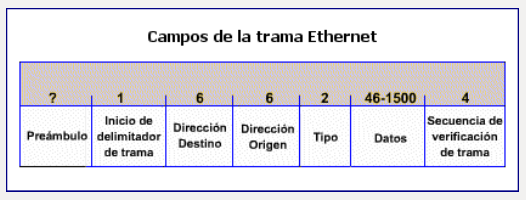
\includegraphics[width=\columnwidth]{./media/image1.png}}
	
	\begin{itemize}		
		\item Preámbulo: Patrón de unos y ceros que indica a las estaciones receptoras que una trama es Ethernet o IEEE 802.3. La trama Ethernet incluye un byte adicional que es el equivalente al campo Inicio de Trama (SOF) de la trama IEEE 802.3. 
		
		\item Inicio de trama (SOF): Byte delimitador de IEEE 802.3 que finaliza con dos bits 1 consecutivos, y que sirve para sincronizar las porciones de recepción de trama de todas las estaciones de la red. Este campo se especifica explícitamente en Ethernet. 
		
		\item Direcciones destino y origen: Incluye las direcciones físicas (MAC) únicas de la máquina que envía la trama y de la máquina destino. La dirección origen siempre es una dirección única, mientras que la de destino puede ser de broadcast única (trama enviada a una sola máquina), de broadcast múltiple (trama enviada a un grupo) o de broadcast (trama enviada a todos los nodos). 
		
		\item Tipo (Ethernet): Especifica el protocolo de capa superior que recibe los datos una vez que se ha completado el procesamiento Ethernet. 
		
		\item Longitud (IEEE 802.3): Indica la cantidad de bytes de datos que sigue este campo. 
		
		\item Datos: Incluye los datos enviados en la trama. En las especificación IEEE 802.3, si los datos no son suficientes para completar una trama mínima de 64 bytes, se insertan bytes de relleno hasta completar ese tamaño (tamaño mínimo de trama). Por su parte, las especificaciones Ethernet versión 2 no especifican ningún relleno, Ethernet espera por lo menos 46 bytes de datos. 
		
		\item Secuencia de verificación de trama (FCS): Contiene un valor de verificación CRC (Control de Redundancia Cíclica) de 4 bytes, creado por el dispositivo emisor y recalculado por el dispositivo receptor para verificar la existencia de tramas dañadas. 
		Cuando un paquete es recibido por el destinatario adecuado, les retira la cabecera de Ethernet y el checksum de verificación de la trama, comprueba que los datos corresponden a un mensaje IP y entonces lo pasa a dicho protocolo para que lo procese. El tamaño máximo de los paquetes en las redes Ethernet es de 1500 bytes.
		
	\end{itemize}
	
	\subsection{Acceso al Medio para Medios Compartidos}
	
	Algunas topologías de red comparten un medio común con varios nodos. En cualquier momento puede haber una cantidad de dispositivos que intentan enviar y recibir datos utilizando los medios de red. Hay reglas que rigen cómo esos dispositivos comparten los medios.   
	
	Hay dos métodos básicos de control de acceso al medio para medios compartidos:
	
	\begin{itemize}
		\item \textbf{Controlado}: Cada nodo tiene su propio tiempo para utilizar el medio
		\item \textbf{Basado en la contención}: Todos los nodos compiten por el uso del medio 
	\end{itemize}
	
	\subsubsection{Acceso controlado para medios compartidos}
	
	Al utilizar el método de acceso controlado, los dispositivos de red toman turnos, en secuencia, para acceder al medio. A este método se lo conoce como acceso programado o determinista. Si un dispositivo no necesita acceder al medio, la oportunidad de utilizar el medio pasa al siguiente dispositivo en línea. Cuando un dispositivo coloca una trama en los medios, ningún otro dispositivo puede hacerlo hasta que la trama haya llegado al destino y haya sido procesada por el destino.  
	
	Aunque el acceso controlado está bien ordenado y provee rendimiento predecible, los métodos determinísticos pueden ser ineficientes porque un dispositivo tiene que esperar su turno antes de poder utilizar el medio.
	
	\subsubsection*{Token Ring}
	Es una arquitectura de red desarrollada por \textbf{IBM} en los años 1970 con topología lógica en anillo y técnica de acceso de paso de testigo, usando un frame de 3 bytes llamado token que viaja alrededor del anillo. Token Ring se recoge en el estándar IEEE 802.5. En desuso por la popularización de Ethernet; actualmente no es empleada en diseños de redes.
	
	\noindent\makebox[\textwidth]{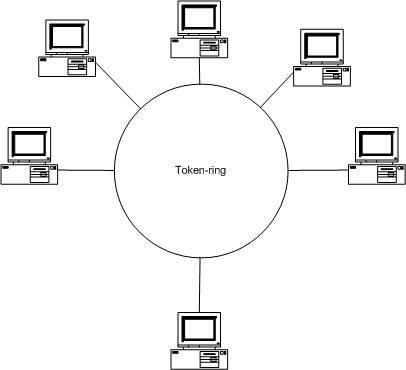
\includegraphics[width=\columnwidth]{./media/image2.png}}
	
	\subsubsection{Acceso por contención para medios compartidos}
	
	Estos métodos por contención, también llamados no deterministas, permiten que cualquier dispositivo intente acceder al medio siempre que haya datos para enviar. Para evitar caos completo en los medios, estos métodos usan un proceso de Acceso múltiple por detección de portadora (CSMA) para detectar primero si los medios están transportando una señal. Si se detecta una señal portadora en el medio desde otro nodo, quiere decir que otro dispositivo está transmitiendo. Cuando un dispositivo está intentando transmitir y nota que el medio está ocupado, esperará e intentará después de un período de tiempo corto. Si no se detecta una señal portadora, el dispositivo transmite sus datos. Las redes \textbf{Ethernet e inalámbricas utilizan control de acceso al medio por contención}.
	
	Es posible que el proceso CSMA falle si dos dispositivos transmiten al mismo tiempo. A esto se lo denomina colisión de datos. Si esto ocurre, los datos enviados por ambos dispositivos se dañarán y deberán enviarse nuevamente.   Los métodos de control de acceso al medio por contención no tienen la sobrecarga de los métodos de acceso controlado. No se requiere un mecanismo para analizar quién posee el turno para acceder al medio. Sin embargo, los sistemas por contención no escalan bien bajo un uso intensivo de los medios. A medida que el uso y el número de nodos aumenta, la probabilidad de acceder a los medios con éxito sin una colisión disminuye. Además, los mecanismos de recuperación requeridos para corregir errores debidos a esas colisiones disminuyen aún más el \textit{throughput}.
	
	CSMA es generalmente implementado junto con un método para resolver la contención del medio. Los dos métodos comúnmente utilizados son:  
	
	\begin{itemize}
		\item \textbf{CSMA/Detección de colisión}   
		En CSMA/Detección de colisión (CSMA/CD), el dispositivo monitorea los medios para detectar la presencia de una señal de datos. Si no hay una señal de datos, que indica que el medio está libre, el dispositivo transmite los datos. Si luego se detectan señales que muestran que otro dispositivo estaba transmitiendo al mismo tiempo, todos los dispositivos dejan de enviar e intentan después. Las formas tradicionales de Ethernet usan este método
		
		\item \textbf{CSMA/Prevención de colisiones}   
		En CSMA/Prevención de colisiones (CSMA/CA), el dispositivo examina los medios para detectar la presencia de una señal de datos. Si el medio está libre, el dispositivo envía una notificación a través del medio, sobre su intención de utilizarlo. El dispositivo luego envía los datos. Este método es utilizado por las tecnologías de redes inalámbricas 802.11.
	\end{itemize}
	
	\subsection{Acceso al Medio para medios no compartidos}
	Los protocolos de control de acceso al medio para medios no compartidos requieren poco o ningún control antes de colocar tramas en los medios. Estos protocolos tienen reglas y procedimientos más simples para el control de acceso al medio. Tal es el caso de las topologías punto a punto.  
	
	En las topologías punto a punto, los medios interconectan sólo dos nodos. En esta configuración, los nodos no necesitan compartir los medios con otros \textit{hosts} ni determinar si una trama está destinada para ese nodo. Por lo tanto, los protocolos de capa de enlace de datos hacen poco para controlar el acceso a medios no compartidos.
	
	En conexiones punto a punto, la Capa de enlace de datos tiene que considerar si la comunicación es \textit{\textbf{half-duplex o fullduplex}}.  
	
	\subsubsection{Duplex Completo}
	
	En la comunicación \textit{full-duplex}, los dos dispositivos pueden transmitir y recibir en los medios al mismo tiempo. La capa de enlace de datos supone que los medios están disponibles para transmitir para ambos nodos en cualquier momento. 
	
	Por lo tanto, no hay necesidad de arbitraje de medios en la capa de enlace de datos.
	
	Una simple ilustración de un sistema de comunicación full-duplex sirve como resumen claro.
	
	\noindent\makebox[\textwidth]{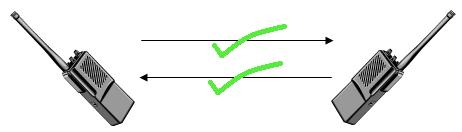
\includegraphics[width=\columnwidth]{./media/image3.JPG}}
	
	La mayoría de los sistemas y redes de comunicaciones modernos funcionan en modo dúplex permitiendo canales de envío y recepción simultáneos. Podemos conseguir esa simultaneidad de varias formas:
	\begin{itemize}
		\item Empleo de frecuencias separadas (multiplexación en frecuencia)
		\item Cables separados
	\end{itemize}
	Nota: Por definición no deben existir colisiones en Ethernet en el modo \textit{full-duplex} (dúplex-completo) aunque inusualmente existen.
	
	\subsubsection{Duplexación por división de tiempo}
	
	La duplexación por división de tiempo (Time-Division Duplexing, TDD) es una técnica para convertir un canal simplex en un canal dúplex separando las señales enviadas y recibidas en intervalos de tiempos diferentes sobre el mismo canal usando acceso múltiple por división de tiempo.
	
	La duplexación por división de tiempo tiene una gran ventaja en los casos en los que hay asimetría entre la velocidad del uplink y el downlink. Según aumenta la cantidad de data en el uplink, más capacidad de comunicación puede ser destinada a este, y si por el contrario el tráfico se vuelve más ligero, se puede reducir su capacidad. Lo mismo puede hacerse con el downlink.
	
	Para sistemas de radio que no se mueven rápidamente, otra ventaja es que la ruta de las ondas del uplink y el downlink son muy similares. Esto significa que técnicas como la formación de rayo trabajan bien con sistemas TDD.
	
	Ejemplos de duplexación por división de tiempo son:
	
	\begin{itemize}
		\item Las interfaces suplementarias de UMTS 3G, TD-CDMA para telecomunicaciones en interiores.
		\item El TD-LTE 4G chino, la interfase para comunicaciones móviles TD-SCDMA 3G.
		\item La telefonía inalámbrica DECT.
		\item Las redes de paquetes semidúplex basadas en acceso múltiple por detección de portadora, por ejemplo ethernet de dos cables o ethernet a través de un concentrador, redes de área local inalámbricas y bluetooth, pueden ser consideradas como sistemas de duplexación por división de tiempo, aunque no TDMA con marcos de ancho fijo.
		\item IEEE 802.16 WiMAX
		\item PACTOR
	\end{itemize}
	
	\subsubsection{Duplexación por división de frecuencia}
	
	La duplexación por división de frecuencia (Frequency-Division Duplexing, FDD) significa que el transmisor y el receptor operan a diferentes frecuencias portadoras. El término es usado frecuentemente entre los radio aficionados, donde un operador está tratando de contactar un repetidor. La estación debe ser capaz de enviar y recibir al mismo tiempo, y hace esto alterando ligeramente la frecuencia a la que envía y recibe. Este modo de operación es referido como modo dúplex o modo complemento.
	
	Se dice que las sub-bandas de uplink y downlink están separadas por el complemento de frecuencia. La duplexación por división de frecuencia puede ser eficiente en el caso de tráfico simétrico. En este caso la duplexación por división de tiempo tiende a desperdiciar ancho de banda durante el cambio de transmisión a recepción, tiene una mayor latencia inherente, y puede requerir circuitería más compleja.
	
	Otra ventaja de la duplexación por división de frecuencia es que hace el planeamiento de radio mucho más fácil y más eficiente, porque las estaciones bases no se "escuchan" entre ellas (transmiten y reciben en diferentes sub-bandas) y por lo tanto normalmente no se interfieren entre ellas. Otra ventaja de la duplexación en frecuencia sobre la de tiempo es que en la duplexación por división de tiempo se deben usar tiempos de guardia entre estaciones bases vecinas (lo que decrementa la eficiencia en el uso del espectro) o se necesita sincronizar estaciones bases, para que puedan transmitir y recibir al mismo tiempo (lo que incrementa la complejidad y por lo tanto el costo, y reduce la flexibilidad de uso de ancho de banda porque todas las estaciones bases y sectores estarán forzados a usar la misma relación uplink/downlink).
	
	Ejemplos de sistemas de duplexación por división de frecuencia son:
	
	\begin{itemize}
		\item ADSL y VDSL
		\item La mayoría de los sistemas celulares, incluyendo el modo de duplexación por división de frecuencia UMTS/WCDMA y el sistema CDMA2000.
		\item El modo de duplexación por división de frecuencia del IEEE 802.16 WiMAX.
	\end{itemize}
	
	\subsubsection{SemiDuplex}	
	Comunicación \textit{half-duplex} quiere decir que los dispositivos pueden transmitir y recibir en los medios pero no pueden hacerlo simultáneamente. Ethernet ha establecido reglas de arbitraje para resolver conflictos que surgen de instancias donde más de una estación intenta transmitir al mismo tiempo.
	
	\noindent\makebox[\textwidth]{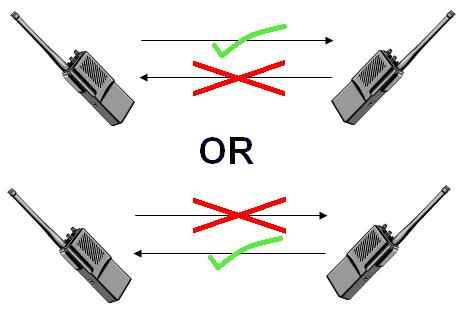
\includegraphics[width=\columnwidth]{./media/image4.JPG}}
	
	Una conexión semidúplex (a veces denominada una conexión alternada) es una conexión en la que los datos fluyen en una u otra dirección, pero no las dos al mismo tiempo. Con este tipo de conexión, cada extremo de la conexión transmite uno después del otro. Este tipo de conexión hace posible tener una comunicación bidireccional utilizando toda la capacidad de la línea. Puede darse el caso de una comunicación por equipos de radio, si los equipos no son full dúplex, uno no podría transmitir (hablar) si la otra persona está también transmitiendo (hablando) porque su equipo estaría recibiendo (escuchando) en ese momento. En radiodifusión, se da por hecho que todo duplex ha de poder ser bidireccional y simultáneo, pues de esta manera, se puede realizar un programa de radio desde dos estudios de lugares diferentes.
	\subsubsection{Simplex}
	Únicamente permiten la transmisión en un sentido (unidireccional). Es aquel en el que una estación siempre actúa como fuente y la otra siempre como receptor. Es el más sencillo y el menos costoso de los tres. Un ejemplo típico es el caso de la fibra óptica; en estos casos se puede recurrir a sistemas en anillo o con doble fibra para conseguir una comunicación completa. Aunque en la actualidad ya existe la posibilidad de enviar y recibir señal a través de una sola fibra óptica pero en diferentes longitudes de onda.
	
	\section{C.S.M.A. (acceso múltiple con escucha de portadora)}
	Acceso Múltiple con Escucha de Señal Portadora (Carrier-Sense Multiple Access o CSMA por sus siglas en ingles) es un protocolo de control de acceso al medio en el cual un nodo verifica la ausencia de trafico antes de transmitir en un medio compartido como un canal electrónico o una banda de espectro electromagnético.
	
	Un transmisor intenta determinar si existe otra transmisión en progreso antes de iniciar una transmisión usando un mecanismo de escucha de señal portadora. Intenta detectar la presencia de una señal portadora de otro nodo antes de intentar transmitir. Si una señal es detectada, el nodo espera a que la transmisión en progreso finalice antes de iniciar su propia transmisión. Usando CSMA, múltiples nodos pueden enviar y recibir por el mismo medio. Transmisiones de un nodo son generalmente recibidas por todos los otros nodos conectados al medio.
	
	Distintas variaciones de CSMA incluyen técnicas de prevención de colisiones, detección de colisiones y resolución de colisiones.
	
	\noindent\makebox[\textwidth]{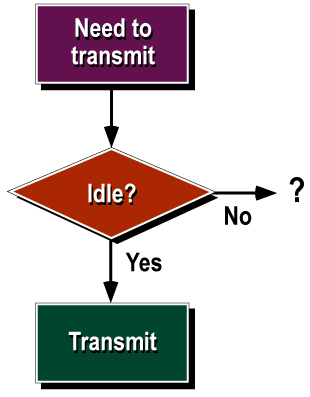
\includegraphics[width=\columnwidth]{./media/image5.jpg}}
	
	\subsection{Detección de Colisiones (CSMA/CD)}
	acceso múltiple con escucha de portadora y detección de colisiones, es un algoritmo de acceso al medio compartido. Su uso está especialmente extendido en redes Ethernet donde es empleado para mejorar sus prestaciones. En CSMA/CD, los dispositivos de red escuchan el medio antes de transmitir, es decir, es necesario determinar si el canal y sus recursos se encuentran disponibles para realizar una transmisión. Además, mejora el rendimiento de CSMA finalizando el envío cuando se ha detectado una colisión. 
	
	\subsubsection{Funcionamiento general}
	
	En CSMA/CD, cada estación que desea transmitir debe realizar una escucha del medio –detección de portadora– para comprobar si éste se encuentra libre, es decir, para comprobar que ninguna otra estación está en ese instante transmitiendo un mensaje. Si el medio se encuentra libre entonces tiene lugar dicha transmisión. Aun así, puede ocurrir que varias estaciones tengan mensajes para enviar y que comiencen a transmitir una trama en el mismo instante. Cuando esto se sucede, se dice que ha ocurrido una colisión en la red. La estación que ha detectado la colisión procederá a enviar un mensaje de \textit{jam} de 32 bits al resto de estaciones para notificar dicho evento. Una vez que todas las estaciones han sido notificadas, automáticamente se paran todas las transmisiones y se ejecuta un algoritmo de backoff (o de postergación) que consiste en esperar un tiempo aleatorio (backoff) antes de volver a intentar la transmisión. Durante los 10 primeros intentos el valor medio del tiempo de espera se duplica mientras que durante los 6 siguientes intentos adicionales, se mantiene. Tras 16 intentos fallidos, el algoritmo notificará un error a las capas superiores.
	
	
	\begin{center}
		\vfill
		\noindent\makebox[\textwidth]{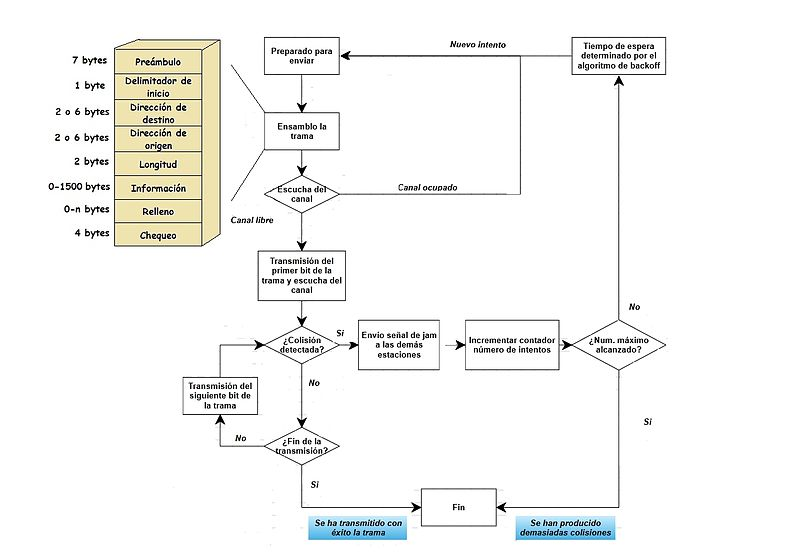
\includegraphics[width=1.8\columnwidth]{./media/image6.jpg}}
	\end{center}
	
	\begin{itemize}
		
		\item Ventajas
		\begin{itemize}
			\item La detección de colisiones en redes LAN cableadas es fácil.
			\item El tiempo medio necesario para detectar una colisión es relativamente bajo.
			\item Puede ser empleado en sistemas de control de procesos continuos si la carga de tráfico de la red es baja (inferior al 20 %)
			\item Ofrece un rendimiento mayor en especial cuando existen pocas colisiones.
		\end{itemize}
		
		\item Desventajas
		\begin{itemize}
			\item Una de las desventajas más importantes radica en que no es posible garantizar un tiempo máximo finito para el acceso de las tramas al canal de comunicación, por lo cual no resulta adecuado para aplicaciones de tiempo real.
			\item Normalmente las redes CSMA/CD son de tipo half-duplex, lo cual significa que mientras una estación envía información es incapaz de escuchar el tráfico existente.
			\item Problemática en redes inalámbricas (ver más abajo)
		\end{itemize}
		
	\end{itemize}
	
	\subsubsection{Trama de CSMA/CD}
	
	La trama empleada en CSMA/CD está formada por ocho campos:
	
	\begin{enumerate}
		\item \textbf{El preámbulo}, formado por 7 octetos, es el encargado de que el receptor pueda sincronizarse con el emisor, de forma que pueda localizarse el principio de la trama.
		
		\item \textbf{Delimitador de inicio}: es un byte empleado para indicar al receptor el inicio de la trama.
		
		\item \textbf{Dirección de destino}: contiene la dirección física (MAC) del equipo destinatario de la trama.
		
		\item \textbf{Dirección de origen}: contiene la dirección MAC de la estación emisora de la trama y tiene un formato similar al de la dirección de destino.
		
		\item \textbf{Longitud}: indica la longitud del campo de datos que se encuentra a continuación. Es necesaria para determinar la longitud del campo de datos en los casos que se utiliza un campo de relleno.
		
		\item \textbf{Información}: contiene los datos transmitidos. Es de longitud variable, por lo que puede tener cualquier longitud entre 42 y 1500 bytes.
		
		\item \textbf{Relleno}: es usado para que la trama alcance la longitud mínima requerida. Una trama debe contener un mínimo número de bytes para que las estaciones puedan detectar las colisiones con precisión.
		
		\item \textbf{Chequeo}: contiene un código de redundancia cíclica de 32 bits. Es utilizada como mecanismo de control de errores en la transmisión.
	\end{enumerate}
	
	\noindent\makebox[\textwidth]{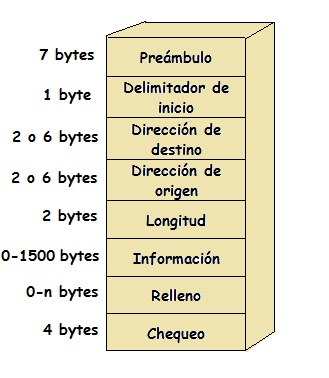
\includegraphics[width=1.2\columnwidth]{./media/image8.jpg}}
	
	\subsubsection{Tipos}
	
	\begin{itemize}
		\item \textbf{CSMA 1-persistente}: cuando una estación quiere transmitir, primero escucha el canal. Si éste está libre entonces transmite inmediatamente. En el caso contrario permanece a la escucha hasta que esté libre. En el momento en el que la estación considere que el canal está disponible, se transmite inmediatamente. El problema radica en que varias estaciones pueden estar esperando a que el canal esté libre para transmitir, dando lugar a una colisión de sus tramas.
		
		\item \textbf{CSMA no persistente}: funciona de forma análoga al anterior excepto en el hecho de que cuando detecta que el canal está ocupado, en vez de permanecer a la espera escuchándolo, espera un tiempo aleatorio y vuelve a escuchar el canal. Con este método se reducen las colisiones si el tráfico es elevado, mejorándose la utilización del canal. Sin embargo aumentan los retardos para cargas de tráfico bajas .
		
		\item \textbf{CSMA p-persistente}: al igual que en los casos anteriores se escucha el canal, sin embargo si éste está libre, en vez de transmitir inmediatamente, se transmite con una probabilidad p, o bien se retrasa la emisión una ranura temporal con una probabilidad q=1-p . Esta ranura temporal suele ser igual al máximo retardo de propagación de la señal.
		
		Habitualmente suele ser utilizado el algoritmo 1-persistente, pues es empleado en el estándar \textbf{IEEE\_802.3}.
	\end{itemize}
	
	\subsubsection{Problemática en redes inalámbricas}
	
	\subsubsection*{Problema del nodo oculto}
	
	En las redes inalámbricas proceder a la escucha del medio y por lo tanto detectar las colisiones producidas, puede resultar complicado. Esto se manifiesta en dos problemáticas:
	
	Problema del nodo oculto: una estación puede creer que el canal (medio) está libre cuando en realidad está ocupado por otra estación a la que no oye. En la siguiente imagen se muestra como A y C transmiten hacia B ya que ambos detectaron que el canal estaba libre. Sin embargo B escucha a ambos nodos, dando lugar a una colisión.
	
	\noindent\makebox[\textwidth]{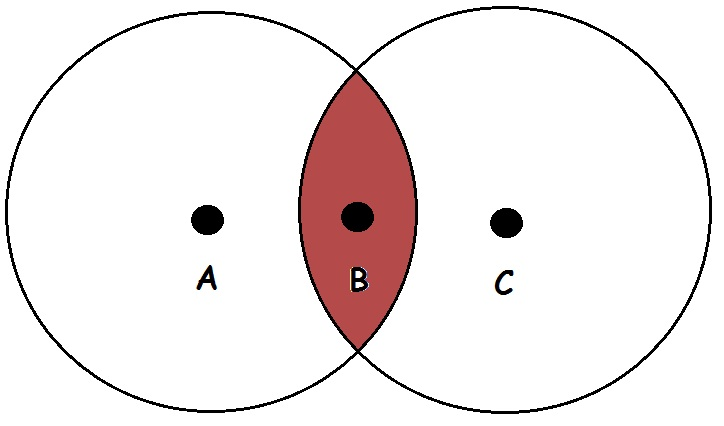
\includegraphics[width=\columnwidth]{./media/image7.jpg}}
	
	\subsubsection*{Problema del nodo expuesto}
	
	Problema del nodo expuesto: una estación puede creer que el canal está ocupado cuando en realidad lo está ocupando otra estación que no interferiría en su transmisión a otro destino. En la figura se muestra como C está comunicándose con B. Como D detecta que el canal está ocupado, no puede transmitir hacia E, cuando lo idóneo sería que sí pudiese.
	
	\noindent\makebox[\textwidth]{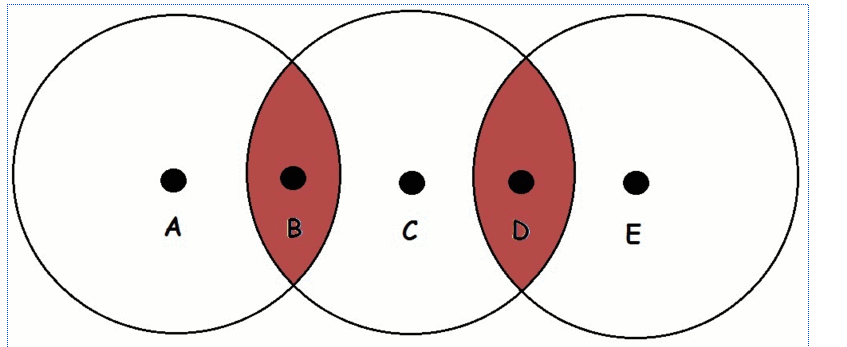
\includegraphics[width=\columnwidth]{./media/image8.png}}
	
	Estos problemas fueron resueltos con la implementación del algoritmo CSMA/CA (MultiAccess Collision Avoidance) 
	
	\subsection{Prevención de Colisiones (CSMA/CA)}
	CSMA/CA (del inglés \textit{Carrier Sense Multiple Access with Collision Avoidance}) o, en español, acceso múltiple por detección de portadora y prevención de colisiones, es un protocolo de control de acceso a redes de bajo nivel que permite que múltiples estaciones utilicen un mismo medio de transmisión. Cada equipo anuncia opcionalmente su intención de transmitir antes de hacerlo para evitar colisiones entre los paquetes de datos (comúnmente en redes inalámbricas, ya que estas no cuentan con un modo práctico para transmitir y recibir simultáneamente). De esta forma, el resto de equipos de la red sabrán cuando hay colisiones y en lugar de transmitir la trama en cuanto el medio está libre, se espera un tiempo aleatorio adicional corto y solamente si, tras ese corto intervalo el medio sigue libre, se procede a la transmisión reduciendo la probabilidad de colisiones en el canal. CSMA/CA es utilizada en canales en los que por su naturaleza no se puede usar CSMA/CD. CSMA/CA se utiliza en 802.11 basada en redes inalámbricas.
	
	Aunque CSMA/CD y CSMA/CA aseguren que un nodo va a obtener un acceso al medio no se asegura que el nodo destino esté en contacto con el nodo origen. Para solucionar este problema se ha añadido un procedimiento de saludo adicional al protocolo de la capa MAC. Este procedimiento se ha denominado protocolo de MAC inalámbrico de fundamento distribuido (DFW MAC) con el fin de que sirva para los diferentes métodos de la capa MAC.
	
	\subsubsection{Funcionamiento}
	
	Para enviar una trama, el equipo origen primero envía una trama corta de control de solicitud de transmisión RTS (Request To Send) mediante el método CSMA/CD o CSMA/CA. Este mensaje de control RTS contiene las direcciones de MAC del equipo origen y destino. Si el equipo destino recibe esta trama significa que está preparado para recibir una trama. Este equipo devolverá una trama de contestación: preparado para transmitir CTS (Clear To Send) o receptor ocupado (RxBUSY). Si la respuesta es afirmativa el equipo origen transmite la trama en espera (DATA). Si el equipo destino recibe correctamente el mensaje contesta con la trama de confirmación positiva ACK (ACKnowledged) y si no la recibe correctamente contesta con la trama de confirmación negativa NAK (NAKnowledged) y el equipo origen tratará de volver a enviarlo. Este procedimiento se repite un número predefinido de veces hasta conseguirse una transmisión correcta de la trama DATA.
	
	A continuación se muestra un esquema general de este procedimiento. 
	
	\noindent\makebox[\textwidth]{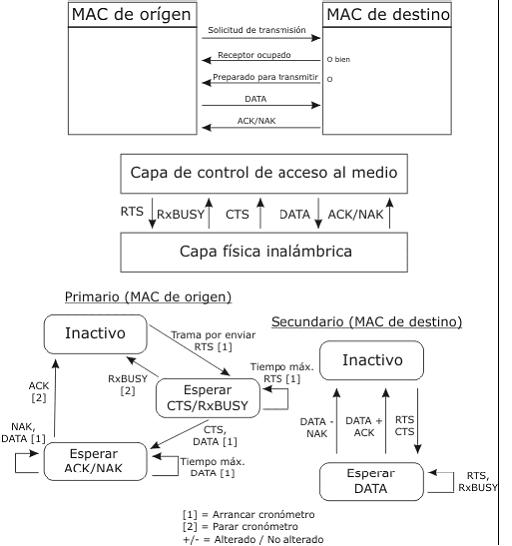
\includegraphics[width=\columnwidth]{./media/image9.JPG}}
	
	Básicamente, este proceso se puede dividir en tres fases en las que el emisor:
	
	\begin{enumerate}
		\item Escucha para ver si la red está libre.
		\item Transmite el dato.
		\item Espera un reconocimiento por parte del receptor.
	\end{enumerate}
	
	
	Este método asegura así que el mensaje se recibe correctamente. Sin embargo, debido a las dos transmisiones, la del mensaje original y la del reconocimiento del receptor, pierde un poco de eficiencia. Este sistema incrementa el volumen de tráfico en el cable y reduce las prestaciones de la red, motivo por el que se usa poco. En redes inalámbricas, no se puede escuchar a la vez que se trasmite: no pueden detectarse colisiones. 
	
	\subsubsection{Problemas que resuelve CSMA/CA (con respecto a CSMA/CD)}
	
	\begin{itemize}
		\item \textbf{Nodos ocultos}: Una estación cree que el canal está libre, pero en realidad está ocupado por otro nodo al que no escucha.
		
		\item \textbf{Nodos expuestos}: Una estación cree que el canal está ocupado, pero en realidad está libre pues el nodo al que escucha no le interferiría. 
	\end{itemize}
	
	\section{Hardware de Comunicación}
	
	\section{Pilas de Protocolos}
	\subsection{O.S.I.}
	\subsection{T.C.P./I.P.}
	
	
	
	
\end{document}
